\documentclass[10pt]{article}  

\usepackage[catalan]{babel}
\usepackage[utf8]{inputenc}  
\usepackage{graphicx}
\usepackage{color}
\definecolor{gray97}{gray}{.97}
\definecolor{gray75}{gray}{.75}
\definecolor{gray45}{gray}{.45}
\usepackage{float}
\usepackage{caption}
\usepackage{listings}
%% CODE %%
\lstset{ frame=Ltb,
framerule=0pt,
aboveskip=0.5cm,
framextopmargin=3pt,
framexbottommargin=3pt,
framexleftmargin=0.4cm,
framesep=0pt,
rulesep=.4pt,
backgroundcolor=\color{gray97},
rulesepcolor=\color{black},
%
stringstyle=\ttfamily,
showstringspaces = false,
basicstyle=\small\ttfamily,
commentstyle=\color{gray45},
keywordstyle=\bfseries,
%
numbers=left,
numbersep=15pt,
numberstyle=\tiny,
numberfirstline = false,
breaklines=true,
}

% minimizar fragmentado de listados
\lstnewenvironment{listing}[1][]
{\lstset{#1}\pagebreak[0]}{\pagebreak[0]}

\lstdefinestyle{consola}
{basicstyle=\scriptsize\bf\ttfamily,
backgroundcolor=\color{gray75},
}

\lstdefinestyle{C}
{language=C,
}
%%%%%%%%%%
\usepackage{anysize}
\marginsize{2cm}{2cm}{2cm}{2cm} % Izquierda, derecha, arriba, abajo

\usepackage[colorlinks=true,plainpages=true,citecolor=blue,linkcolor=black,urlcolor=blue]{hyperref}

% Para agregar encabezado y pie de página
\usepackage{fancyhdr} 
\pagestyle{fancy}
\fancyhf{}
\fancyhead[L]{\footnotesize XARXES I COMUNICACIONS} %encabezado izquierda
\fancyhead[R]{\footnotesize EPS-UdL}   % dereecha
\fancyfoot[R]{\footnotesize Pràctica 3}  % Pie derecha
\fancyfoot[C]{\thepage}
\fancyfoot[L]{\footnotesize Grau en Enginyeria Informàtica}  %izquierda
\renewcommand{\footrulewidth}{0.4pt}

%%%%%%%% TERMINA PREÁMBULO %%%%%%%%%%%%

\begin{document}
\thispagestyle{empty}

%%%%%%%%%%%%%%%%%%%%%%%%%%%%%%%%%% PORTADA %%%%%%%%%%%%%%%%%%%%%%%%%%%%%%%%%%%%%%%%%%%%
                                                                                    %%%
\begin{center}                                                                      %%%
\newcommand{\HRule}{\rule{\linewidth}{0.5mm}}                                   %%%\left
                                                                                    %%%
\begin{minipage}{0.48\textwidth} \begin{flushleft}

\includegraphics[scale = 0.23]{Images/logo_udl.jpg}
\end{flushleft}\end{minipage}
\begin{minipage}{0.48\textwidth} \begin{flushright}

\includegraphics[scale = 0.25]{Images/logo_eps.jpg}
\end{flushright}\end{minipage}

                                                                                    %%%
\vspace*{-1.5cm}                                %%%
                                                                                    %%% 
\textsc{\huge ESCOLA POLIT\` ECNICA \\ \vspace{5px}SUPERIOR}\\[1.5cm] 

\textsc{\LARGE XARXES I COMUNICACIONS}\\[1.5cm]                                                   %%%

\begin{minipage}{0.9\textwidth} 
\begin{center}                                                                                  %%%
\textsc{\LARGE PR\`ACTICA 3}
\end{center}
\end{minipage}\\[0.5cm]
%%%
                                                                                    %%%
            \vspace*{1cm}                                                                       %%%
                                                                                    %%%
\HRule \\[0.4cm]                                                                    %%%
{ \huge \bfseries Full Redundant SLB \& SNMP}\\[0.4cm]  %%%
                                                                                    %%%
\HRule \\[1.5cm]                                                                    %%%
                                                                                %%%
                                                                                    %%%
\begin{minipage}{0.46\textwidth}                                                    %%%
\begin{flushleft} \large                                                            %%%
\emph{Students:}\\   
Nil Agut Marín\\
Jaume Giralt Barbé
%%%
            %\vspace*{2cm}  
                                                                %%%
                                                                %%%
\end{flushleft}                                                                     %%%
\end{minipage}      
                                                                %%%
\begin{minipage}{0.52\textwidth}        
\vspace{-0.6cm}                                         %%%
\begin{flushright} \large                                                           %%%
\emph{Professor:} \\                                                                 %%%
Fernández Camon, Cèsar                                                    %%%
\end{flushright}                                                                    %%%
\end{minipage}  
\vspace*{1cm}
%\begin{flushleft}
    

\begin{center}                                                                                  
{\large \today}                                                                 %%%
            \end{center}                                                                        
\end{center}                                                                        
                                                                                    
\newpage                                                                        
%%%%%%%%%%%%%%%%%%%% TERMINA PORTADA %%%%%%%%%%%%%%%%%%%%%%%%%%%%%%%%

\tableofcontents
\listoffigures 

\newpage
\section{Objectius}
L'objectiu principal d'aquesta pràctica és implementar \textbf{SLB} i \textbf{SNMP}.
\section{Full Redundant SLB}
\subsection{Topologia de la xarxa}
\begin{figure}[H]
\begin{center}
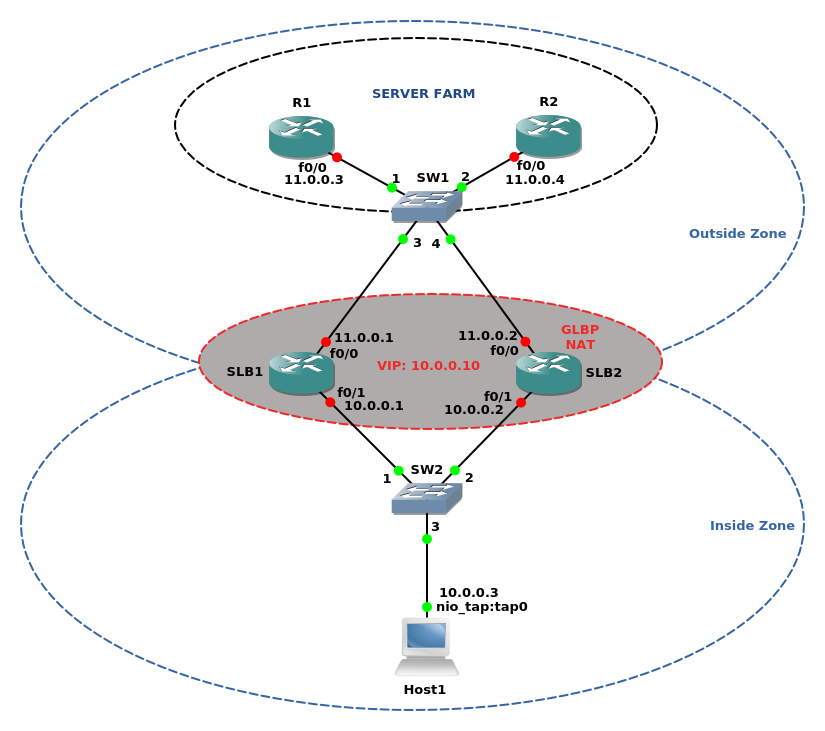
\includegraphics[scale=0.6]{Images/topology1.png}
\caption{SLB - Topologia de la xarxa a efectuar l'exercici}
\end{center}
\end{figure}
Per a la realització de aquest exercici utilitzarem encaminadors \textbf{Cisco c7200}
\subsection{Principals problemes de configuració i com ho hem solucionat}
El principal problema que hem tingut en la realització d'aquesta pràctica ha sigut la connexió amb la \textit{Server Farm} mitjançant el protocol HTTPS. Hem aconseguit realitzar connexions mitjançant el protocol HTTP al server farm. També hem aconseguit la redundància entre els dos encaminadors SLB i si un enllaç o un servidor fallava del server farm, el altre servidor responia. 
\\\\
Com hem dit anteriorment, el gran problema d'aquest apartat han sigut les connexions HTTPs per culpa dels certificats. El primer problema amb el qual ens vam trobar va ser que el protocol scp no és podia utilitzar en aquests encaminadors. Vam intentar exportar els certificats a la memòria del router, la nvram. Tot i així, no eram capaços d'importar els certificats. També hem intentat amb altres protocols com el tftp. Hem instal·lat el paquet i ens hem intentat connectar al servidor. Hem configurat el servei tftp, afegint \textit{-c} al camp TFTP\underline{ }OPTIONS per tal de poder crear arxius encara que no estiguessin. Hem configurat al encaminador que utilitzen el protocol SLB les següents comandes:
\begin{itemize}

\item[- ]\textit{crypto pki trustpoint TP}
\item[- ]\textit{subject-name O=Test,CN=xarxes-lab.cat}
\item[- ]\textit{rsakeypair XARXES-KEY}
\item[- ]\textit{enrollment selfsigned}
\item[- ]\textit{revocation-check none}
\item[- ]\textit{crypto key generate rsa general-keys label XARXES-KEY modulus 1024\ exportable}
\item[- ]\textit{crypto pki enroll TP}
\item[- ]\textit{crypto pki export TP pem url tftp: des PASSWORD }
\item[- ]\textit{ip http secure-trustpoint TP}
\item[- ]\textit{ip http secure-server}
\end{itemize}
Tot i així, quan intentem connectar-nos al servidor tftp que tenim en el nostre ordinador, no connecta. Hem pensat que podria ser per que faltessin rutes estàtiques, les hem posat però continua sense funcionar.
\section{Proves de connexió}
En les següents dues captures podem veure que en cas que un dels dos servidors de la granja caigués, l'altre ocuparia el seu lloc i respondria a la petició del client. Per tant, tenim redundància. Ho podem veure en les captures 2 i 3 del document.
\\\\
També podem veure que en les captures 4, 5 i 6, hem apagat el encaminador el qual tenia el estat Actiu i responia les peticions del client, forçant així que l'altre servidor ocupés el seu lloc i pogués respondre les peticions del client.
\begin{figure}
	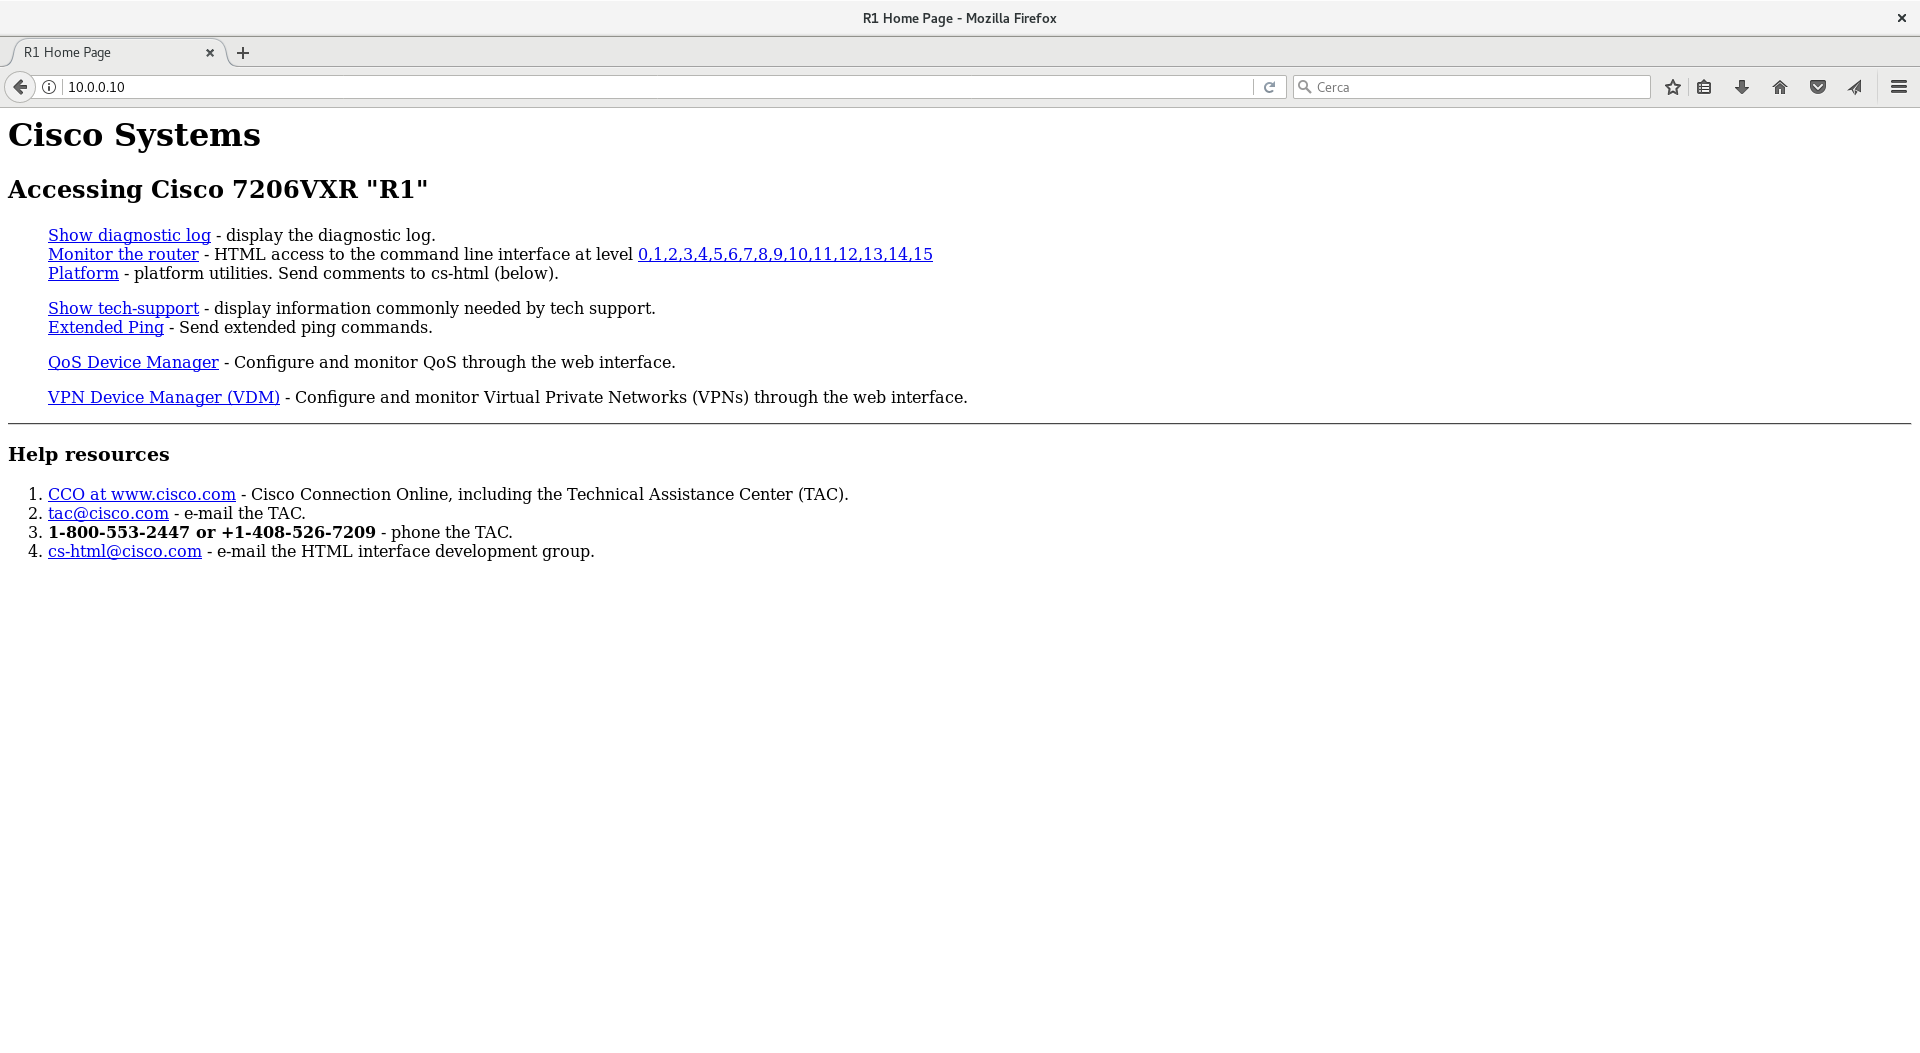
\includegraphics[scale=0.24]{Images/R1.png}
	\caption{Connexions mitjançant el protocol HTTP - R1}
	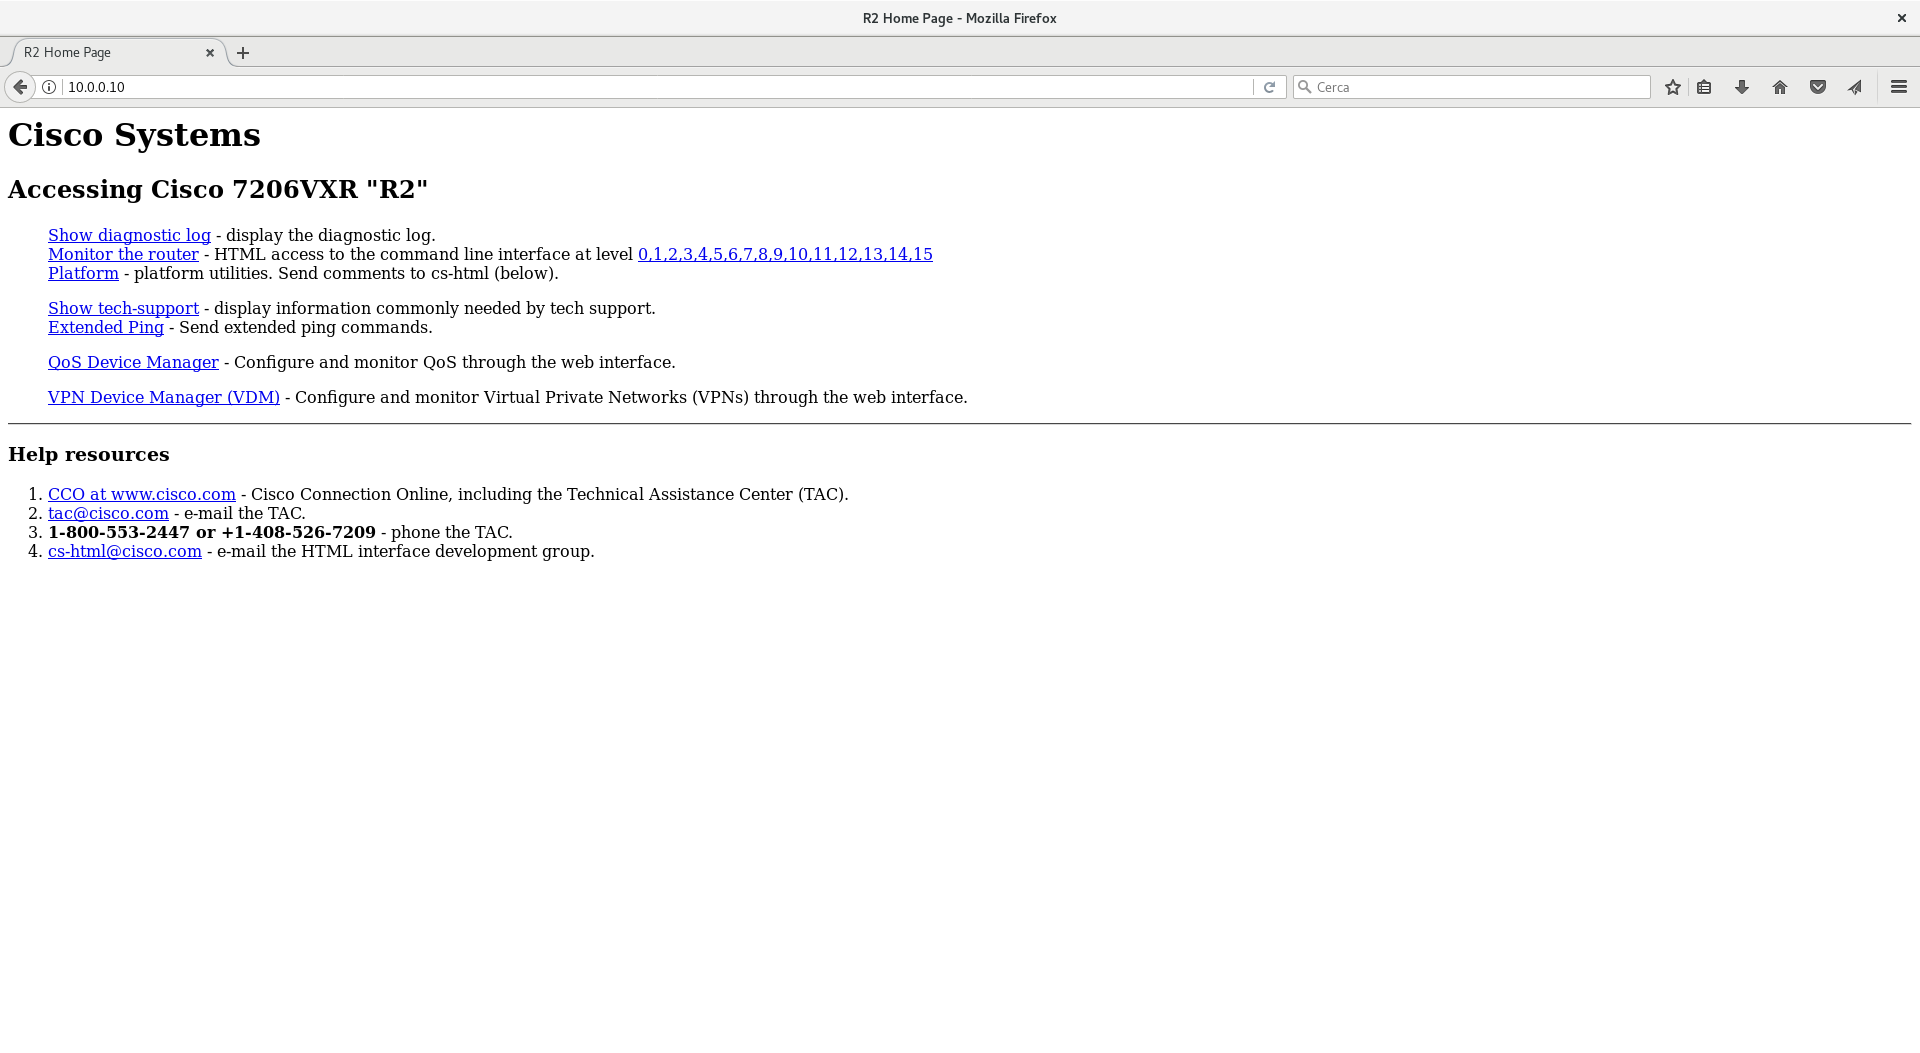
\includegraphics[scale=0.24]{Images/R2.png}
	\caption{Connexions mitjançant el protocol HTTP - R2}
\end{figure}
\begin{figure}
	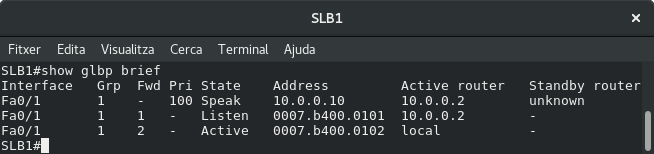
\includegraphics[scale=0.7]{Images/captura1.png}
	\caption{Configuració GLBP SLB1}
	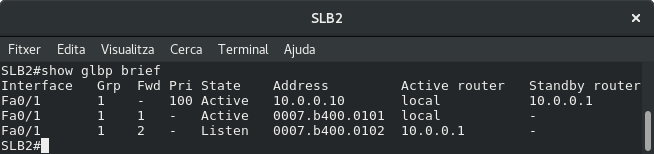
\includegraphics[scale=0.7]{Images/Captura2.png}
	\caption{Configuració GLBP SLB2}
	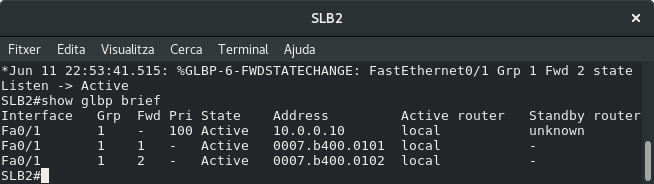
\includegraphics[scale=0.7]{Images/captura3.png}
	\caption{Configuració GLBP SLB2 després caiguda SLB1}
\end{figure}
\newpage
\section{SNMP}
\subsection{Introducció}
A continuació es detallarà la solució implementada per a la gestió de routers mitjançant el protocol snmp. No s'han assolit tots els objectius proposats en l'enunciat de la pràctica. Hem configurat els dos primers objectius correctament i hem intentat fer el graf. Tot i així hem tingut problemes al posar les etiquetes als enllaços.
\\\\
Per a la resolució d'aquest apartat hem tingut que utilitzar la llibreria de snmp-mibs per tal de poder interactuar amb els encaminadors CISCO.
\subsection{Executar el programa}
Les llibreries necessàries per l'execució del programa han sigut les següents:
\begin{itemize}
	\item easysnmp
	\item graphviz
	\item os
	\item optparse
\end{itemize}
\subsection{Estructura del programa}
El programa el composen els següents documents en Python:
\begin{itemize}
	\item part2.py: Lògica de l'executable
	\item utils.py: Classes per a la realització de l'execució.
	\item strings.py: Strings per a l'executable.
\end{itemize}
\subsection{Procediments}
Ara parlarem sobre les funcions més importants per a l'execució del programa:
\begin{itemize}
\item analyze\underline{ }topology(): En aquesta classe recorrerem tota la topologia de la xarxa. Per a cada interfície que trobem, si no l'hem trobat abans, inicialitzarem un objecte Router on guardarem el nom, interfícies, veïns i rutes que té.
\item analyze\underline{ }routers(): Com hem dit en la funció anterior, aquí es crearan els diferents objectes de Router.
\item analyze\underline{ }route(): En aquesta funció s'analitzarà cada ruta que té cada encaminador. Es connectara amb el snmp i ens retornara la llista de ip's fent un walk.
\item analyze\underline{ }route(): En aquesta funció s'analitzarà cada interfície que té cada encaminador. Es connectara amb el snmp i ens retornara la llista de ip's, nom de cada interfície, velocitat.
\item graph\underline{ }creator(): En aquesta funció, es crearà un fitxer amb la topologia de la xarxa. Es creara un arxiu png i un arxiu .dot. Es important que hi hagi permisos d'escriptura en aquella carpeta si no no es podrà executar i guardar la topologia.
\end{itemize}
\end{document}
              
